Dado o caráter multifacetado deste projeto, a compreensão das interações entre seus diversos subsistemas pode apresentar desafios significativos. Com o propósito de simplificar e aprofundar esse processo de compreensão, a figura \ref{fig3:image_17} oferece uma representação visual por meio de um diagrama de blocos que esclarece as dinâmicas entre os distintos subsistemas desenvolvidos. Essa abordagem contribui para facilitar o entendimento holístico do sistema na totalidade, proporcionando um recurso valioso para pesquisadores futuros que desejam explorar e aprimorar este laboratório.


\begin{figure}[!h]
	\centering
	\caption{Diagrama do Laboratório Virtual.}
	\efbox{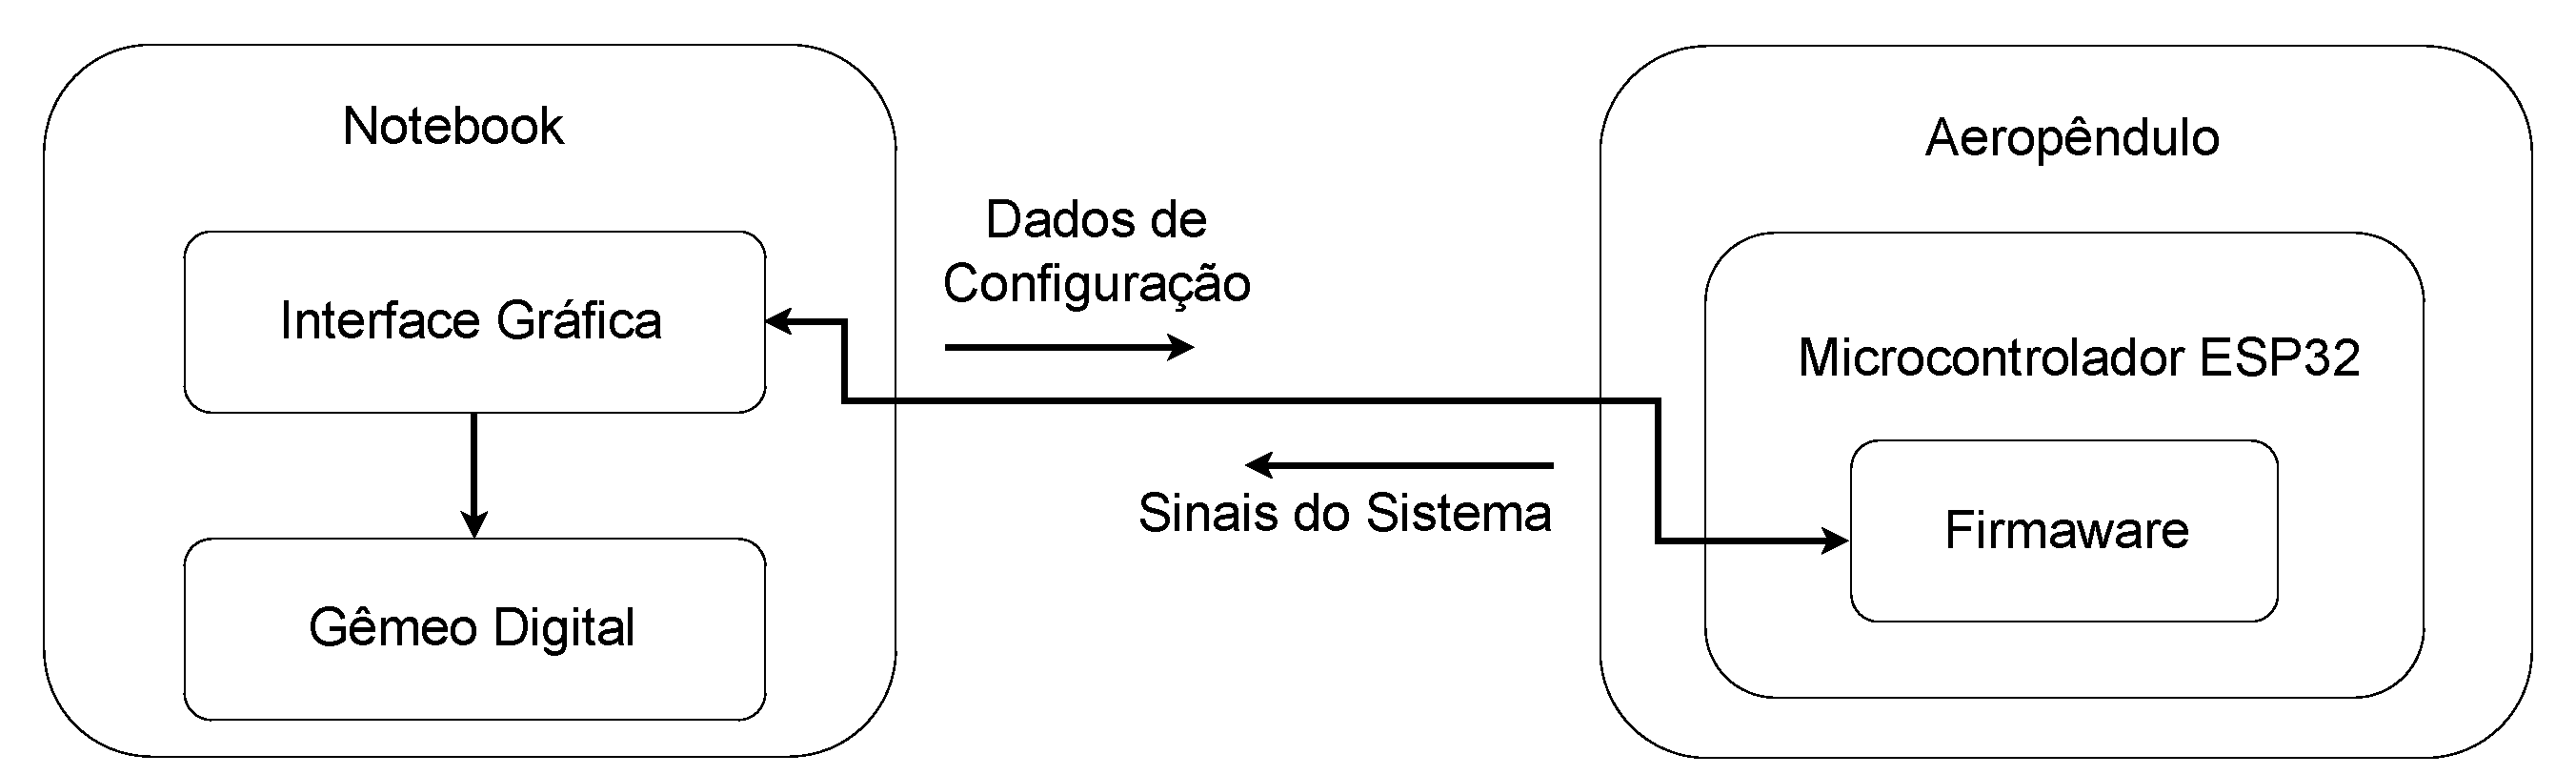
\includegraphics[width=1.0\textwidth]{Capitulos/3_hardware_softwares/3_figuras/diagrama_ecossistema.pdf}}
	\caption*{Fonte: elaborado pelo autor (2023).}
	\label{fig3:image_17}
\end{figure}
